\documentclass[a4paper]{scrreprt}
\usepackage{graphicx}
\usepackage{subfig}

\begin{document}
\chapter{Your Chapter}
Lorem ipsum dolor sit amet, consetetur sadipscing elitr, sed diam 
nonumy eirmod tempor invidunt ut labore et dolore magna aliquyam 
erat, sed diam voluptua. At vero eos et accusam et justo duo dolores 
et ea 
rebum. Stet clita kasd gubergren, no sea takimata sanctus est Lorem 
ipsum dolor sit amet. Lorem ipsum dolor sit amet, consetetur 
sadipscing elitr, sed diam nonumy eirmod tempor invidunt ut labore et
dolore magna aliquyam erat, sed diam voluptua. At vero eos et accusam
et justo duo dolores et ea rebum. Stet clita kasd gubergren, no sea 
takimata sanctus est Lorem ipsum dolor sit amet.

\begin{figure}[ht]
    \centering
    \subfloat[South American coati]{
        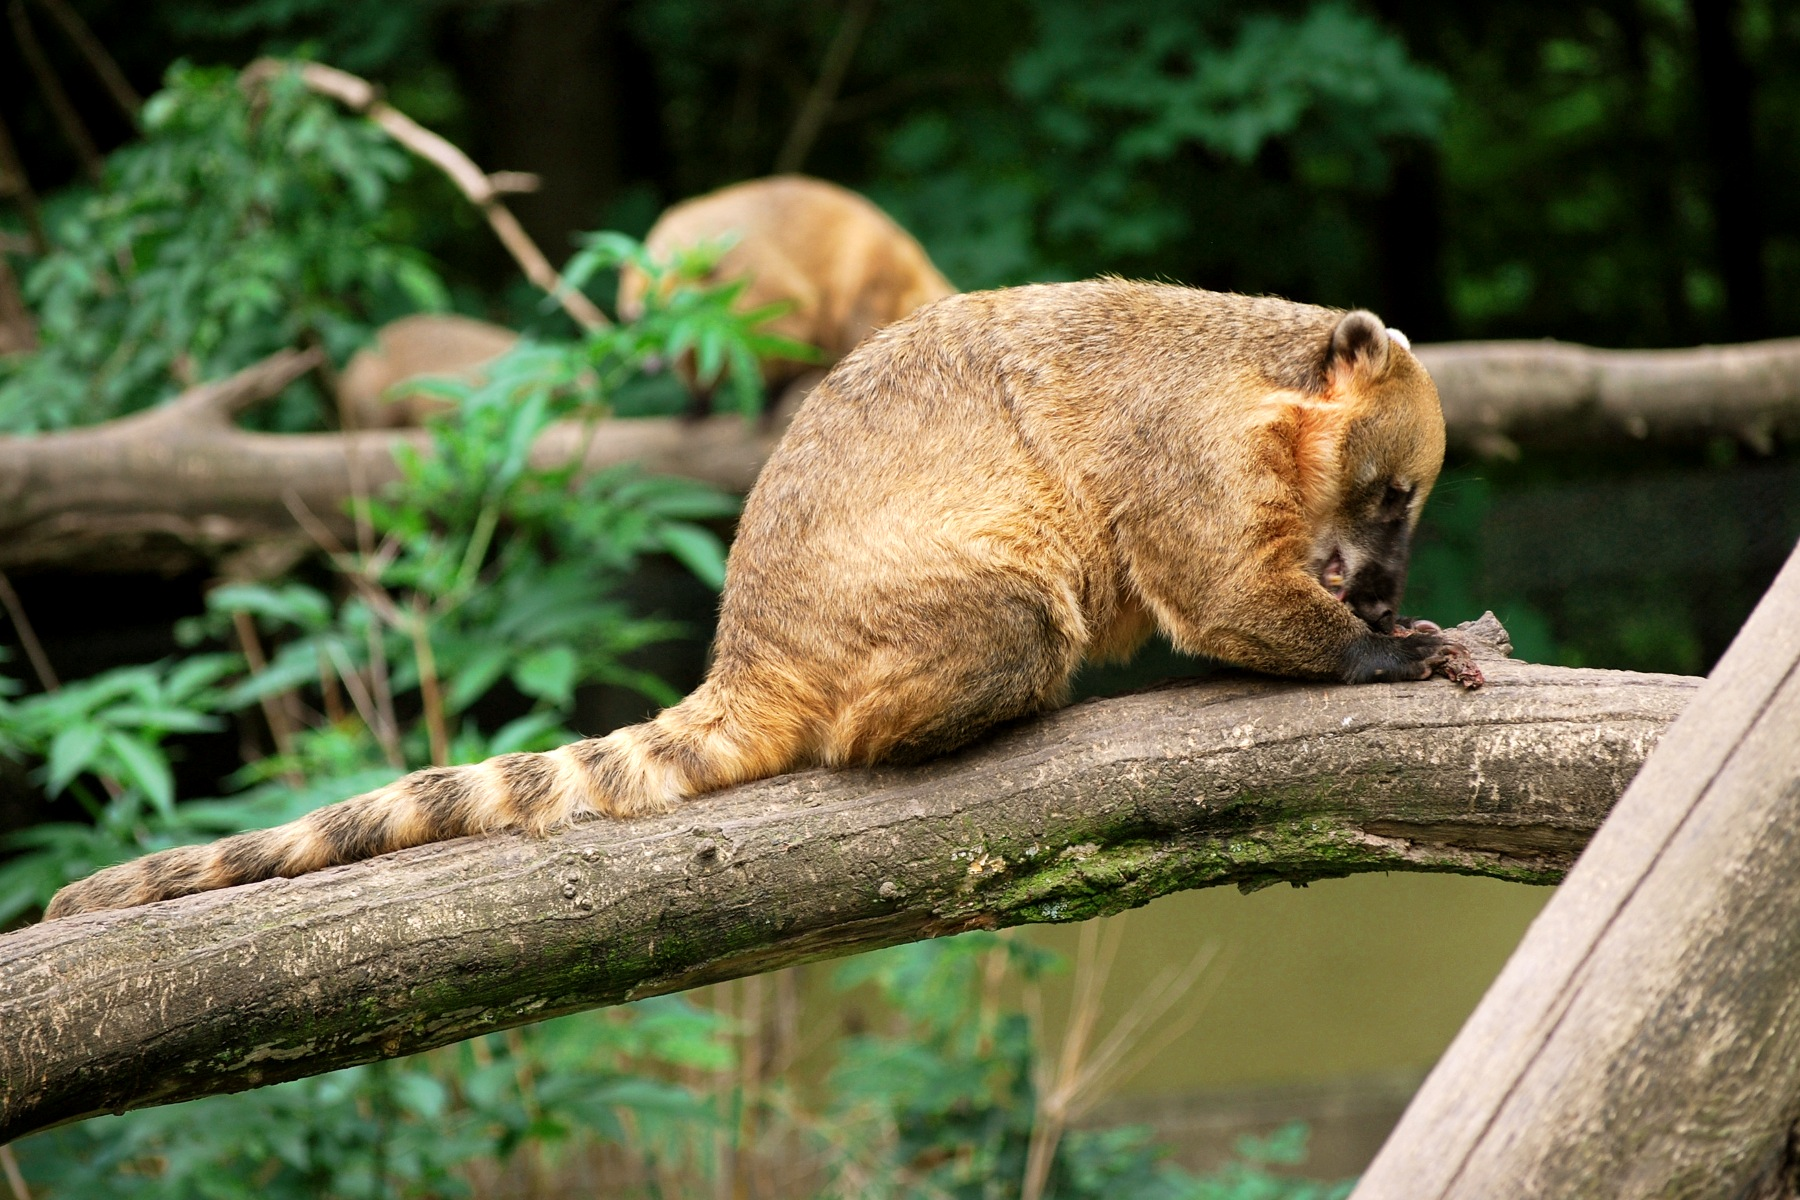
\includegraphics[width=0.45\textwidth]{YourImage.jpg}
        \label{fig:nasua}
    }%
    \subfloat[Brown bear]{
        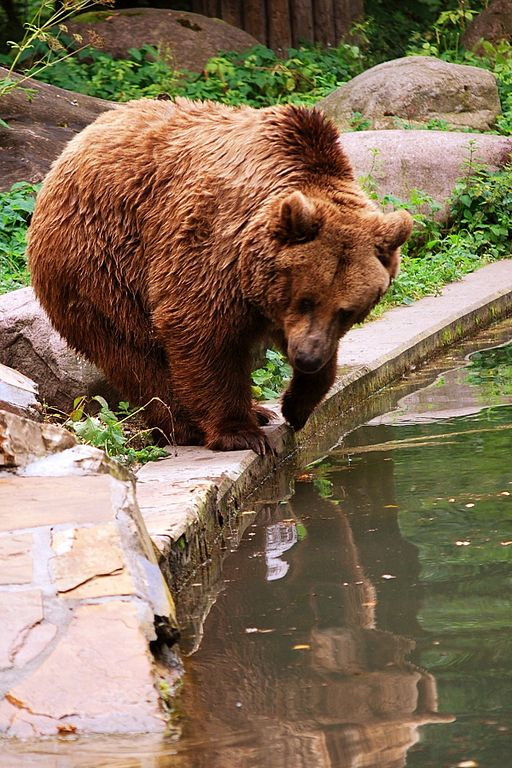
\includegraphics[width=0.45\textwidth]{Ursus-arctos.jpg}
        \label{fig:Ursus-arctos}
    }
    \label{fig:formen}
    \caption{Bears}
\end{figure}

You can now see that a Nasua nasua in figure \ref{fig:nasua} and a Ursus-arctos 
in figure \ref{fig:Ursus-arctos}. Note that you have to run LaTeX twice and
don't delete intermediate files when you want to use ref.

\end{document}
